\section{Case Studies}

In this section, we present representative cases that demonstrate \kimi{3}'s capabilities across diverse technical tasks.

\begin{figure}[t]
  \centering
  \resizebox{\columnwidth}{!}{\begingroup
\definecolor{kernelKimi}{RGB}{243,70,69}
\definecolor{kernelClaude}{RGB}{141,170,211}
\definecolor{kernelGPTFive}{RGB}{155,195,173}
\definecolor{kernelGPTSol}{RGB}{193,103,113}
\definecolor{kernelGrid}{RGB}{239,239,239}
\definecolor{kernelText}{RGB}{64,64,64}
\pgfplotsset{
  relative offsets/.style={
      table/create on use/x/.style={create col/expr accum={\pgfmathaccuma+\thisrow{dx}}{0}},
      table/create on use/y/.style={create col/expr accum={\pgfmathaccuma+\thisrow{dy}}{0}},
    },
}
\begin{tikzpicture}
  \begin{axis}[
      scale only axis=true,
      width=12.6cm, height=5.6cm,
      xmin=-0.19, xmax=24,
      ymin=0, ymax=64.1,
      axis x line*=bottom, axis y line*=left,
      axis line style={draw=black,line width=.6pt},
      tick style={draw=black,line width=.5pt},
      major tick length=2.5pt,
      xtick={0,5,10,15,20},
      ytick={0,10,20,30,40,50,60,64.1},
      tick label style={font=\small,text=black},
      xlabel={Active hours},
      ylabel={Speedup vs. FLA Triton Baseline (\%)},
      label style={font=\small,text=black},
      ymajorgrids=true, xmajorgrids=false,
      grid style={draw=kernelGrid,line width=.5pt},
      clip=false,
      unbounded coords=discard,
    ]
    \addplot[draw=kernelClaude,opacity=.3,dashed,line width=0.7pt,mark=none]
    table[relative offsets,x=x,y=y] {
        dx dy
        -0.19 57.12
        24 0
      };
    \addplot[draw=kernelGPTFive,opacity=.3,dashed,line width=0.7pt,mark=none]
    table[relative offsets,x=x,y=y] {
        dx dy
        -0.19 30.76
        24 0
      };
    \addplot[draw=kernelGPTSol,opacity=.3,dashed,line width=0.7pt,mark=none]
    table[relative offsets,x=x,y=y] {
        dx dy
        -0.19 17.34
        24 0
      };
    \addplot[draw=kernelKimi,opacity=.3,dashed,line width=0.7pt,mark=none]
    table[relative offsets,x=x,y=y] {
        dx dy
        -0.19 59.66
        24 0
      };
    \addplot[only marks,mark=x,mark size=1.45pt,mark options={draw=kernelClaude,opacity=.4,line width=.65pt}]
    table[relative offsets,x=x,y=y] {
        dx dy
        5.34 2.56
        0.09 7.88
        4.75 29.32
        2.93 15.52
      };
    \addplot[only marks,mark=x,mark size=1.7pt,mark options={draw=kernelClaude,opacity=.5,line width=.75pt}]
    table[relative offsets,x=x,y=y] {
        dx dy
        4.97 0
        0.95 26.68
        0.18 -3.42
        0.1 -1.01
        0.21 -22.25
        2.62 29.47
        0.2 -10.2
        0.17 4.97
        0.15 7.97
        1.37 -3.33
        1.66 26.26
        0.3 -0.38
      };
    \addplot[only marks,mark=x,mark size=1.45pt,mark options={draw=kernelGPTFive,opacity=.4,line width=.65pt}]
    table[relative offsets,x=x,y=y] {
        dx dy
        0.45 0
        0.21 0
        0.16 0
        0.07 0
        0.12 0
        0.11 0
        0.53 0
        0.03 0
        0.42 0
        0.15 0
        0.07 0
        0.39 0.02
        0.09 0
        0.15 0.06
        0.1 0.2
        0.05 -0.01
        0.16 0.02
        0.04 0.12
        0.81 0.03
        2.54 9.82
        6.65 19.17
        0.66 0.05
        1.45 0.39
        0.25 0.1
        0.22 -0.24
      };
    \addplot[only marks,mark=x,mark size=1.7pt,mark options={draw=kernelGPTFive,opacity=.5,line width=.75pt}]
    table[relative offsets,x=x,y=y] {
        dx dy
        0.78 0
        0.42 0
        0.73 0
        0.15 0
        0.11 0
        0.36 0
        0.23 0.01
        0.23 -0.01
        0.13 0.09
        0.03 -0.07
        0.04 -0.02
        0.13 0
        0.08 0
        0.04 0.44
        0.03 -0.11
        0.04 -0.33
        0.04 0
        0.04 0.16
        0.03 0.25
        0.03 -0.09
        0.03 0.05
        0.03 0.06
        0.04 -0.43
        0.03 0.35
        0.04 0.09
        0.03 -0.02
        0.03 -0.04
        0.04 -0.38
        0.08 0.3
        0.04 -0.07
        0.03 0.18
        0.09 -0.41
        0.03 0.43
        0.17 -0.43
        0.07 0.34
        0.2 0.43
        0.07 -0.77
        0.07 0.82
        0.07 0.01
        0.05 -0.08
        0.04 -0.01
        1 9.57
        0.23 0.06
        0.06 0.1
        0.14 -0.16
        0.06 0.03
        0.05 0.02
        0.12 0.04
        0.23 -1.43
        0.24 1.49
        0.04 -0.22
        0.04 0.13
        0.02 0.1
        0.03 -0.12
        0.03 -0.78
        0.04 0.86
        0.04 0
        0.05 -0.02
        0.03 -0.21
        0.02 0.01
        0.02 0.08
        0.02 -0.29
        0.02 0.3
        0.08 0.13
        0.08 -0.02
        0.03 -0.19
        0.21 -1.62
        0.07 2.21
        0.08 -0.17
        0.51 -4.5
        0.08 5.2
        0.07 -0.31
        0.07 0.86
        0.08 -0.01
        0.24 -0.27
        0.05 0.25
        0.21 -0.84
        0.35 1.77
        0.12 0.06
        0.09 0.21
        0.05 -0.13
        0.06 0.08
        0.05 -0.13
        0.08 0.09
        0.06 0.08
        0.06 -0.04
        0.08 -0.81
        0.05 0.82
        0.08 -0.45
        0.02 0.36
        0.02 -0.17
        0.08 0.21
        0.08 -0.13
        0.03 0.07
        0.53 -12.91
        0.09 29.45
        0.02 0.02
        0.07 -1.78
        0.03 -0.14
        0.04 1.78
        0.04 0.05
        0.03 -6.99
        0.03 4.9
        0.03 1.36
        0.03 -2.2
        0.03 -5.96
        0.04 -20.49
        0.06 22.35
        0.03 6.15
        0.13 0.77
        0.03 0.3
        0.04 -0.57
        0.03 0.46
        0.04 -5.31
        0.06 5.35
        0.06 -0.14
        0.04 0.09
        0.12 -2.9
        0.04 -6.69
        0.04 8.72
        0.04 -0.93
        0.11 -0.42
        0.08 2.32
        0.15 -0.42
        0.04 -0.07
        0.04 0.34
        0.04 -0.13
        0.08 -3.55
        0.08 2.76
        0.08 0.49
        0.07 -15.97
        0.15 16.51
        0.14 0.06
        0.08 -2.46
        0.08 2.36
        0.16 -0.09
        0.21 0.02
        0.05 0.08
        0.05 -0.05
        0.08 -0.08
        0.05 -0.05
        0.03 0.15
        0.03 -0.24
        0.03 0.09
        0.03 -0.7
        0.04 0.92
        0.04 -9.25
        0.04 6.83
        0.04 1.4
        0.04 0.86
        0.04 -3.71
        0.1 -25.39
        0.07 21.59
        0.06 4.94
        0.04 2.68
        0.04 -1.6
        0.02 -0.61
        0.1 2.56
        0.09 0
        0.04 0.03
        0.02 -0.13
        0.05 0
        0.04 0.11
        0.02 0.01
        0.02 -0.05
        0.06 -0.01
        0.02 -0.77
        0.1 0.78
        0.16 0.08
        0.07 -5.03
        0.07 2.85
        0.02 1.51
        0.04 0.68
        0.06 -0.16
        0.06 0
        0.03 0.13
        0.02 -0.05
        0.09 -6.29
        0.04 5.96
        0.07 -0.78
        0.04 1.18
        0.29 -0.55
        0.04 1
        0.14 -3.64
        0.06 1.17
        0.04 -27.85
        0.06 30.67
        0.04 -0.14
        0.07 0.04
        0.03 -0.11
        0.15 0.07
        0.12 0.11
        0.04 -0.16
        0.04 0.16
        0.06 -0.01
        0.02 -0.1
        0.03 0
        0.06 -0.36
        0.06 0.34
        0.03 -0.13
        0.07 0.16
        0.02 0.05
        0.03 -0.04
        0.02 0.01
        0.03 0.1
        0.06 -0.14
        0.02 0.12
        0.06 -0.09
        0.02 0.08
        0.03 -0.16
        0.02 0.05
        0.09 0.17
        0.02 0.02
        0.03 -7.17
        0.02 7.09
        0.03 -0.96
        0.02 1
        0.07 -0.13
        0.05 -0.02
        0.02 0.05
        0.02 0.06
        0.03 -0.25
        0.08 0.15
        0.06 -0.04
        0.03 0
        0.02 0.04
        0.02 0.16
        0.03 -0.2
        0.03 -0.33
        0.06 0.42
        0.03 -0.12
        0.03 0.19
        0.03 -0.06
        0.03 0.11
        0.03 -0.17
        0.06 -0.12
        0.04 0.16
        0.06 0.01
        0.04 -0.48
        0.03 0.44
        0.04 -0.05
        0.02 -0.04
        0.05 0.12
        0.03 -0.05
        0.03 0.02
        0.03 -0.07
        0.04 0.09
        0.03 0.1
        0.04 -0.04
        0.03 -0.05
        0.07 0.01
        0.12 0.09
        0.05 -0.02
        0.08 0.01
        0.03 -0.13
        0.02 -0.62
        0.03 0.57
        0.02 0.23
        0.02 0.04
        0.03 -0.61
      };
    \addplot[only marks,mark=x,mark size=1.45pt,mark options={draw=kernelGPTSol,opacity=.4,line width=.65pt}]
    table[relative offsets,x=x,y=y] {
        dx dy
        8.46 0
        2.29 6.86
      };
    \addplot[only marks,mark=x,mark size=1.7pt,mark options={draw=kernelGPTSol,opacity=.5,line width=.75pt}]
    table[relative offsets,x=x,y=y] {
        dx dy
        16.01 14.31
        3.39 2.06
      };
    \addplot[only marks,mark=x,mark size=1.45pt,mark options={draw=kernelKimi,opacity=.4,line width=.65pt}]
    table[relative offsets,x=x,y=y] {
        dx dy
        7.92 48.44
        2.32 0.21
        5.07 5.01
      };
    \addplot[only marks,mark=x,mark size=1.7pt,mark options={draw=kernelKimi,opacity=.5,line width=.75pt}]
    table[relative offsets,x=x,y=y] {
        dx dy
        1.02 0
      };
    \addplot[const plot mark left,draw=kernelClaude,line width=0.8pt,mark=*,mark size=1.2pt,mark options={fill=kernelClaude,draw=kernelClaude}]
    table[relative offsets,x=x,y=y] {
        dx dy
        0 0
        4.16 15.67
        1.18 0
        0.09 0
        0 4.01
        0.07 7.03
        1.03 0.61
        2.34 2.39
        0.26 1.63
        0.02 0.89
        0.58 1.71
        0.23 3.01
        0.11 2.81
        0.11 0
        1.06 5.46
        0.15 7.14
        0.1 1.49
        0.35 1.46
        1.27 0
        0.24 0.61
        0.17 0.77
        1.82 0.43
      };
    \addplot[const plot mark left,draw=kernelGPTFive,line width=0.8pt,mark=*,mark size=1.2pt,mark options={fill=kernelGPTFive,draw=kernelGPTFive}]
    table[relative offsets,x=x,y=y] {
        dx dy
        0 0
        0.14 0.43
        0.31 0
        0.21 0
        0.16 0
        0.07 0
        0.12 0
        0.11 0
        0.53 0
        0.03 0
        0.42 0
        0.15 0
        0.07 0
        0.39 0
        0.09 0
        0.15 0
        0.1 0
        0.05 0
        0.16 0
        0.04 0
        0.08 0.06
        0.73 0
        0.41 0.38
        0.51 0.04
        0.54 5.15
        0.25 4.32
        0.2 0.18
        0.63 0
        1.16 0.29
        0.63 1.19
        0.56 0.3
        0.27 0.33
        0.21 0.32
        0.14 0.02
        0.11 0.08
        1.42 3.55
        0.04 9.11
        0.06 2.9
        0.04 0.83
        0.09 0.05
        0.36 0.04
        0.35 0.02
        1.21 0
        0.66 0
        1.07 0.26
        0.23 0.13
        0.15 0
        0.25 0
        0.22 0
        0.56 0.68
        0.09 0.03
        0.75 0.01
        0.29 0.01
        0.32 0.05
        0.6 0
      };
    \addplot[const plot mark left,draw=kernelGPTSol,line width=0.8pt,mark=*,mark size=1.2pt,mark options={fill=kernelGPTSol,draw=kernelGPTSol}]
    table[relative offsets,x=x,y=y] {
        dx dy
        0 0
        0.47 0.25
        0.19 0.03
        7.8 0
        0.38 0.79
        0.91 5.6
        0.38 0.49
        0.62 0
        0.63 0.74
        0.19 0.89
        0.88 1.24
        0.38 0.74
        0.98 2.57
        0.76 0.38
        0.7 0.66
        1.38 0.24
        1.98 2.05
        1.19 0.67
      };
    \addplot[const plot mark left,draw=kernelKimi,line width=0.8pt,mark=*,mark size=1.2pt,mark options={fill=kernelKimi,draw=kernelKimi}]
    table[relative offsets,x=x,y=y] {
        dx dy
        0 0
        2.37 4.39
        0.23 2.95
        0.4 0.47
        0.21 10.98
        0.17 9.04
        0.15 3.89
        0.37 5.23
        0.52 3.67
        0.93 2.41
        0.2 4.5
        0.3 0.58
        0.84 0.05
        0.37 0.06
        0.57 0.24
        0.29 0
        0.26 0.19
        2.06 0
        1.19 3.28
        0.36 1.88
        0.61 1.01
        0.34 1.55
        0.47 0.62
        0.34 0.06
        0.5 2.6
        0 0.01
        1.26 0
      };
    \addplot[only marks,mark=*,mark size=2.5pt,mark options={fill=kernelKimi,draw=kernelKimi}]
    table[relative offsets,x=x,y=y] {
        dx dy
        22.5 59.66
      };
    \node[anchor=west,font=\scriptsize,text=kernelText] at (axis cs:23,60.3) {Kimi K3 $+59.7\%$};
    \addplot[only marks,mark=*,mark size=2.5pt,mark options={fill=kernelClaude,draw=kernelClaude}]
    table[relative offsets,x=x,y=y] {
        dx dy
        22.5 57.12
      };
    \node[anchor=west,font=\scriptsize,text=kernelText] at (axis cs:23,56.4) {Claude Fable 5 $+57.1\%$};
    \addplot[only marks,mark=*,mark size=2.5pt,mark options={fill=kernelGPTFive,draw=kernelGPTFive}]
    table[relative offsets,x=x,y=y] {
        dx dy
        22.5 30.76
      };
    \node[anchor=west,font=\scriptsize,text=kernelText] at (axis cs:23,30.76) {GPT-5.5 $+30.8\%$};
    \addplot[only marks,mark=*,mark size=2.5pt,mark options={fill=kernelGPTSol,draw=kernelGPTSol}]
    table[relative offsets,x=x,y=y] {
        dx dy
        22.5 17.34
      };
    \node[anchor=west,font=\scriptsize,text=kernelText] at (axis cs:23,17.34) {GPT-5.6 Sol $+17.3\%$};
  \end{axis}
\end{tikzpicture}
\endgroup
}
  \caption{Case study: GPU kernel optimization on AttnRes.}
  \label{fig:case-kernel}
\end{figure}

\begin{figure}[h]
\centering
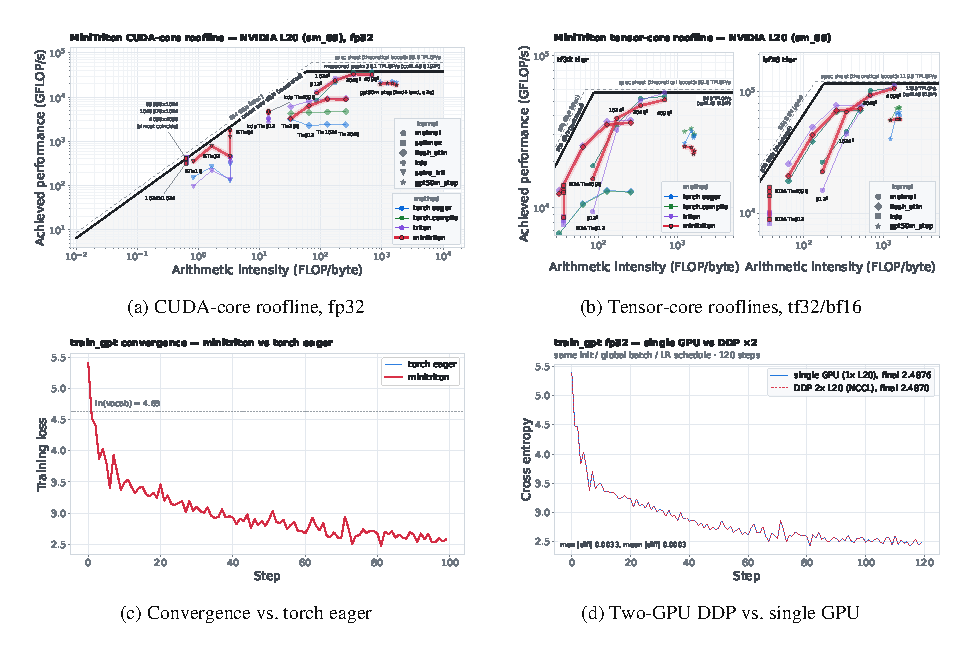
\includegraphics{figures/appendix/minitriton/case-study-compiler.pdf}
\caption{Case study: GPU compiler development with MiniTriton. (a) CUDA-core
and (b) tensor-core rooflines of MiniTriton kernels on an NVIDIA L20 (sm\_89)
against torch eager, torch.compile, Triton, and cuBLAS baselines (losing
points included); (c) training-loss curves of the character-level GPT trained
with MiniTriton versus torch eager; (d) two-GPU data-parallel training built
on MiniTriton's own distributed primitives (NCCL) versus single-GPU training.}
\label{fig:case-compiler}
\end{figure}






\paragraph{GPU kernel optimization}
We tested the models' ability to optimize GPU kernels. Each model works independently in an identically configured sandbox, with a budget of up to 24 hours per task for profiling, rewriting, and benchmarking. The evaluation covers four representative kernels: AttnRes, DeepSeek Sparse Attention (DSA), KDA, and MLA (with head dimension 512), on an NVIDIA Hopper GPU and an alternative-vendor GPGPU.
\kimi{3} substantially improved performance across all four kernels, reducing AttnRes latency from 283.6\,ms to 114.4\,ms, cutting DSA and KDA runtime by 55.1\% and 73.6\%, respectively, and reaching over half of peak TFLOPS on MLA.
Across these tasks, \kimi{3} matched Claude Fable 5~\citep{claudefable5} (with fallback) and substantially outperformed Claude Opus 4.8~\citep{claudeopus48}, GPT-5.6 Sol~\citep{gpt56sol}, and GPT-5.5~\citep{gpt55}.
Figure~\ref{fig:case-kernel} compares the models' optimization trajectories on AttnRes.
Beyond the benchmark, an early \kimi{3} checkpoint was already handling most of our kernel optimization work during late-stage development.


\paragraph{GPU compiler development} \kimi{3} developed MiniTriton\footnote{\url{https://github.com/MoonshotAI/minitriton}}, a compact Triton-like~\citep{tillet2019triton} compiler with a custom tile-level Python frontend and layout system, a lightweight warp-level MLIR~\citep{lattner2021mlir} annotation and optimization layer, and a Parallel Thread Execution (PTX) code-generation pipeline. Built around the compiler is a dual-mode tensor library with a PyTorch-like~\citep{paszke2019pytorch} high-level interface, whose eager and forward-only compiled paths share the same DSL compiler and runtime. The library further provides reverse-mode autograd, neural-network modules, distributed-training primitives over NCCL~\citep{nccl},  and sparse and visualization primitives.
On an NVIDIA L20, MiniTriton outperforms PyTorch eager~\citep{paszke2019pytorch} and \texttt{torch.compile}~\citep{ansel2024pytorch2} in geometric mean over its core benchmark suite. Its from-scratch tensor-core matmul path approaches cuBLAS~\citep{cublas} at the largest shapes,  reaching about 90\% of the measured machine roof, while its DSL-level KDA~\citep{team2025kimi} prefill kernel outperforms a matched Triton reference by a clear margin. MiniTriton also trains a GPT model end to end with a loss curve closely tracking the PyTorch reference, with full-model gradients differing from torch autograd by no more than torch's own fp32 rounding error ($10^{-4}$), measured against an fp64 reference. Together, These results demonstrate that \kimi{3} can build a coherent end-to-end compiler --- from DSL frontend and IR passes to PTX codegen and CUDA runtime --- rather than a collection of isolated kernels (Figure~\ref{fig:case-compiler}).


\paragraph{Chip design} 
As an early proof of concept, \kimi{3} designed an inference-chip prototype for a nano model following the same architecture --- hybrid KDA and NoPE-MLA attention, Block AttnRes with a block size of two, sigmoid-based MoE routing with one shared expert --- under
group-wise INT4 weight quantization (group size 128). In a single 48-hour autonomous run with Kimi Code, \kimi{3} built, optimized, and verified the chip using open-source EDA tools with the Nangate45 standard-cell library~\cite{nangate45}. Within the 4\,mm$^2$ analytical area budget, the design closes timing at 100\,MHz and achieves an RTL-simulated decode throughput of over 8{,}700 tokens/s, integrating 1.46M standard cells, 0.277 MiB of SRAM, and an INT4 MAC array with fused dequantization. 
The RTL code is available on GitHub\footnote{\url{https://github.com/MoonshotAI/nano-kpu}}.



\paragraph{Coding for research} To reproduce the I--Love--Q universal relations in computational astrophysics, \kimi{3} reviewed more than 20 papers and cross-validated their results, implemented the full numerical pipeline, evaluated over 300 equations of state, identified inconsistencies in published formulas, wrote more than 3,000 lines of Python, and produced an interactive HTML dashboard --- in about two hours, versus a typical one to two weeks for an experienced researcher. 

\paragraph{Knowledge work} In Kimi Work, \kimi{3} produced an interactive research website covering 42 years of the AI ASIC industry. The model completed more than 120 rounds of iterative refinement, drawing on a corpus of 87 quarterly reports and 99 original PDFs (more than 11,000 pages) through over 2,800 web searches and over 1,100 terminal queries.
In a second case, \kimi{3} analyzed 391 gravitational-wave events in GWTC-5 using more than 20 concurrent subagents, producing seven scientific visualizations, two summary tables, and a literature synthesis of over ten papers.



\paragraph{Video editing and motion design} Leveraging its native multimodal architecture, \kimi{3} created a 3Blue1Brown-style motion-graphics explainer of its own architecture, and edited its teaser video from 56 source clips. This involved clip selection, motion-matched cuts, frame-accurate beat synchronization, audio processing, and multiple rounds of revision. Producing a comparable high-density short video would typically take an experienced editor one to two days.